\documentclass[problem]{mcs}

\begin{pcomments}
    \pcomment{TP_Bipartite_Graphs}
    \pcomment{Converted from prob6.scm
              by scmtotex and dmj
              on Sun 13 Jun 2010 10:52:29 AM EDT}
\end{pcomments}

\begin{problem}

%% type: short-answer
%% title: Bipartite Graphs

\begin{center}

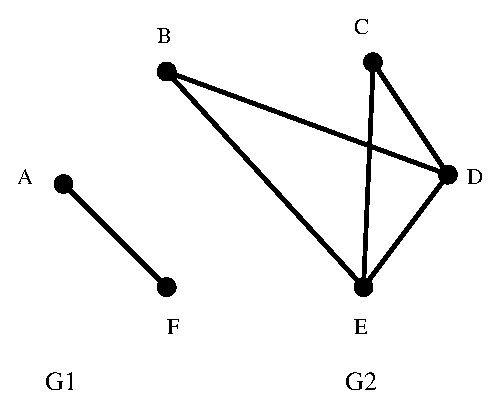
\includegraphics{prob6a} 

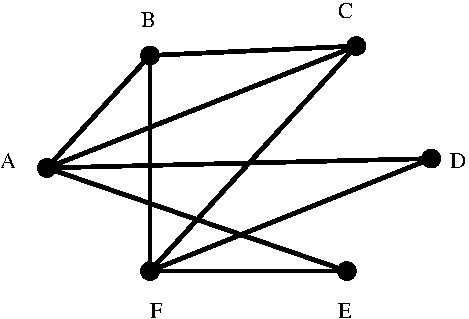
\includegraphics{prob6b}

\includegraphics{prob6c}

\end{center}

Which of the graphs above are bipartite?  

%%  Give your answer as a
%%  sequence of the labels separated by some spaces in any order such as
%%  
%%  \begin{equation*}
%%  b a
%%  \end{equation*}
%%  
%%  Don't use commas or parentheses.

\begin{solution}
a

Graph~a is bipartite: The first color is assigned to the top-left,
bottom-middle, and top-right vertices; the second color is assigned to
the other three vertices.

Graphs b and~c are not bipartite, as they contain cycles of odd
length.
\end{solution}

\end{problem}

\endinput
